\documentclass[]{article}
\setlength{\parskip=0.7}{\baselineskip}
\setlength{\parindent}{0pt}

\usepackage{times}
\usepackage{fullpage}

\usepackage{epsfig}
\usepackage{subfigure}

\usepackage{listings}
\usepackage{siunitx}
\usepackage[super]{nth}
\usepackage{hyperref}


\usepackage{xcolor}
\hypersetup{
    colorlinks,
    linkcolor={red!50!black},
    urlcolor={blue!90!black}
}

\newcommand{\us}{$\mu$s }
\newcommand{\subtopic}[1]{\vspace{1.5pt} \noindent \textit{#1}}

\begin{document}

\title{Kawkab: Distributed Filesystem for Fast Data}
%\author{Sajjad}
\maketitle

\section{Introduction} Kawkab is a distributed filsesystem developed to
efficiently manage large amounts of streaming data.

\section{Architecture} Kawkab mainly follows the same design approach as a
standard Unix filesystem. The metadata of the files is stored separately from
the file data.  The filesystem consists of a file directory, file index,
metadata blocks, and the actual data blocks.

\subsection{File Directory} All the files are referenced through a primary
structure called file directory. A file directory contains the mapping of the
file names to the file index ID.  The index ID is used to search and retrieve
the file index.

\subtopic{File Namespace} Kawkab has a flat namespace. Kawkab does not maintain
directory hierarchies. However, a user can use any file name that can be mapped
to a directory structure. For example, a file name can be "/home/file1.txt.

\subsection{File Index}
File index is the main structure that keeps track of the file metadata and the
index of the data blocks.
The file index stores references to the data blocks in three ways:

\begin{enumerate}
  \item \subtopic{Direct Block:} File index keeps the reference of the first $N$ data blocks of
        the file. The number of direct blocks is kept small to optimize for memory space and file 
        access for small files. The number of direct blocks is fixed and is set as a filesystem 
        parameter.

  \item \subtopic{Indirect Block:} File index has one indirect block that contains
        a large number of direct blocks. If the size of a file exceeds from $N$ blocks, the
        new blocks are added in an indirect block. The number of direct blocks in
        an indirect block is fixed.

  \item \subtopic{Double Indirect Block:} File index has one double indirect block. A
        double indirect block is a two level index: it contains a list of indirect blocks.
        The double indirect block indexes a very large number of blocks that reach the
        file size limit of $2^{63} - 1$ bytes.

\end{enumerate}


\subsection{Data Blocks}

A data block contains the actual file data. Each data block has a fixed size, which can be
set as a filesystem parameter. 

\subsection{File Indexing}

  - How data is indexed

  - How data is retrieved given a byte offset

  - How data is retrieved given a timestamp

\section{Comparison with Existing Systems}

- Comparison with Alluxio

- Comparison with Succinct

- Comparison with HDFS and similar systems

\begin{figure}[t]
    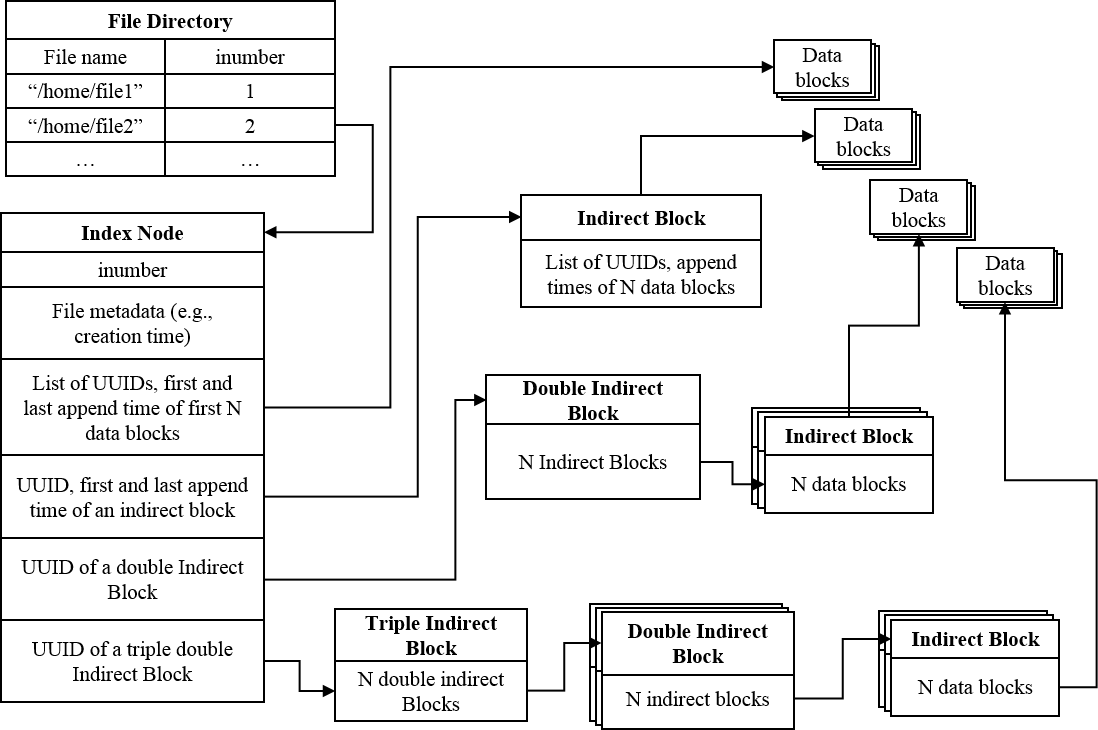
\includegraphics[width=0.9\columnwidth]{{figures/file-index-design.png}}
    \caption{File directory and file index.}
   \label{fig:files-index}
\end{figure}



\end{document}
